\documentclass[11pt]{article}
\usepackage[hidelinks]{hyperref}
\usepackage{tabularx}
\usepackage{graphicx}
\usepackage{adjustbox}
\usepackage[shortlabels]{enumitem}
\usepackage{booktabs}
\usepackage{multirow}

%%%%%%%%%%%%%%%%%%%%%%%%%%%%%%%%%%%%%%%%%
% Lachaise Assignment
% Structure Specification File
% Version 1.0 (26/6/2018)
%
% This template originates from:
% http://www.LaTeXTemplates.com
%
% Authors:
% Marion Lachaise & François Févotte
% Vel (vel@LaTeXTemplates.com)
%
% License:
% CC BY-NC-SA 3.0 (http://creativecommons.org/licenses/by-nc-sa/3.0/)
% 
%%%%%%%%%%%%%%%%%%%%%%%%%%%%%%%%%%%%%%%%%

%----------------------------------------------------------------------------------------
%	PACKAGES AND OTHER DOCUMENT CONFIGURATIONS
%----------------------------------------------------------------------------------------

\usepackage{amsmath,amsfonts,stmaryrd,amssymb} % Math packages

\usepackage{enumerate} % Custom item numbers for enumerations

\usepackage[ruled]{algorithm2e} % Algorithms

\usepackage[framemethod=tikz]{mdframed} % Allows defining custom boxed/framed environments

\usepackage{listings} % File listings, with syntax highlighting
\lstset{
	basicstyle=\ttfamily, % Typeset listings in monospace font
}

%----------------------------------------------------------------------------------------
%	DOCUMENT MARGINS
%----------------------------------------------------------------------------------------

\usepackage{geometry} % Required for adjusting page dimensions and margins

\geometry{
	paper=a4paper, % Paper size, change to letterpaper for US letter size
	top=2.5cm, % Top margin
	bottom=3cm, % Bottom margin
	left=2.5cm, % Left margin
	right=2.5cm, % Right margin
	headheight=14pt, % Header height
	footskip=1.5cm, % Space from the bottom margin to the baseline of the footer
	headsep=1.2cm, % Space from the top margin to the baseline of the header
	%showframe, % Uncomment to show how the type block is set on the page
}

%----------------------------------------------------------------------------------------
%	FONTS
%----------------------------------------------------------------------------------------

\usepackage[utf8]{inputenc} % Required for inputting international characters
\usepackage[T1]{fontenc} % Output font encoding for international characters

\usepackage{XCharter} % Use the XCharter fonts

%----------------------------------------------------------------------------------------
%	COMMAND LINE ENVIRONMENT
%----------------------------------------------------------------------------------------

% Usage:
% \begin{commandline}
%	\begin{verbatim}
%		$ ls
%		
%		Applications	Desktop	...
%	\end{verbatim}
% \end{commandline}

\mdfdefinestyle{commandline}{
	leftmargin=pt,
	rightmargin=10pt,
	innerleftmargin=15pt,
	middlelinecolor=black!50!white,
	middlelinewidth=2pt,
	frametitlerule=false,
	backgroundcolor=black!5!white,
	frametitle={Command Line},
	frametitlefont={\normalfont\sffamily\color{white}\hspace{-1em}},
	frametitlebackgroundcolor=black!50!white,
	nobreak,
}

% Define a custom environment for command-line snapshots
\newenvironment{commandline}{
	\medskip
	\begin{mdframed}[style=commandline]
}{
	\end{mdframed}
	\medskip
}

%----------------------------------------------------------------------------------------
%	FILE CONTENTS ENVIRONMENT
%----------------------------------------------------------------------------------------

% Usage:
% \begin{file}[optional filename, defaults to "File"]
%	File contents, for example, with a listings environment
% \end{file}

\mdfdefinestyle{file}{
	innertopmargin=1.4\baselineskip,
	innerbottommargin=0.5\baselineskip,
	topline=false, bottomline=false,
	leftline=false, rightline=false,
	leftmargin=0cm,
	rightmargin=0cm,
	singleextra={%
		\draw[fill=black!10!white](P)++(0,-1.2em)rectangle(P-|O);
		\node[anchor=north west]
		at(P-|O){\ttfamily\mdfilename};
		%
		\def\l{3em}
		\draw(O-|P)++(-\l,0)--++(\l,\l)--(P)--(P-|O)--(O)--cycle;
		\draw(O-|P)++(-\l,0)--++(0,\l)--++(\l,0);
	},
	nobreak,
}

% Define a custom environment for file contents
\newenvironment{file}[1][File]{ % Set the default filename to "File"
	\medskip
	\newcommand{\mdfilename}{#1}
	\begin{mdframed}[style=file]
}{
	\end{mdframed}
	\medskip
}

%----------------------------------------------------------------------------------------
%	NUMBERED QUESTIONS ENVIRONMENT
%----------------------------------------------------------------------------------------

% Usage:
% \begin{question}[optional title]
%	Question contents
% \end{question}

\mdfdefinestyle{question}{
	innertopmargin=1.2\baselineskip,
	innerbottommargin=0.8\baselineskip,
	roundcorner=5pt,
	nobreak,
	singleextra={%
		\draw(P-|O)node[xshift=1em,anchor=west,fill=white,draw,rounded corners=5pt]{%
		Question \theQuestion\questionTitle};
	},
}

\newcounter{Question} % Stores the current question number that gets iterated with each new question

% Define a custom environment for numbered questions
\newenvironment{question}[1][\unskip]{
	\bigskip
	\stepcounter{Question}
	\newcommand{\questionTitle}{~#1}
	\begin{mdframed}[style=question]
}{
	\end{mdframed}
	\medskip
}

%----------------------------------------------------------------------------------------
%	WARNING TEXT ENVIRONMENT
%----------------------------------------------------------------------------------------

% Usage:
% \begin{warn}[optional title, defaults to "Warning:"]
%	Contents
% \end{warn}

\mdfdefinestyle{warning}{
	topline=false, bottomline=false,
	leftline=false, rightline=false,
	nobreak,
	singleextra={%
		\draw(P-|O)++(-0.5em,0)node(tmp1){};
		\draw(P-|O)++(0.5em,0)node(tmp2){};
		\fill[black,rotate around={45:(P-|O)}](tmp1)rectangle(tmp2);
		\node at(P-|O){\color{white}\scriptsize\bf !};
		\draw[very thick](P-|O)++(0,-1em)--(O);%--(O-|P);
	}
}

% Define a custom environment for warning text
\newenvironment{warn}[1][Warning:]{ % Set the default warning to "Warning:"
	\medskip
	\begin{mdframed}[style=warning]
		\noindent{\textbf{#1}}
}{
	\end{mdframed}
}

%----------------------------------------------------------------------------------------
%	INFORMATION ENVIRONMENT
%----------------------------------------------------------------------------------------

% Usage:
% \begin{info}[optional title, defaults to "Info:"]
% 	contents
% 	\end{info}

\mdfdefinestyle{info}{%
	topline=false, bottomline=false,
	leftline=false, rightline=false,
	nobreak,
	singleextra={%
		\fill[black](P-|O)circle[radius=0.4em];
		\node at(P-|O){\color{white}\scriptsize\bf i};
		\draw[very thick](P-|O)++(0,-0.8em)--(O);%--(O-|P);
	}
}

% Define a custom environment for information
\newenvironment{info}[1][Info:]{ % Set the default title to "Info:"
	\medskip
	\begin{mdframed}[style=info]
		\noindent{\textbf{#1}}
}{
	\end{mdframed}
}
 

\title{AMS 582 Fall 2021\\Design and Analysis of Experiments\\The One-Sixty-Fourth Fraction\\ of the $\pmb{2^{10}}$ Factorial Design}

\author{
  Kai Li\thanks{Department of Applied Mathematics and Statistics, Stony Brook University, email: \href{mailto:kai.li@stonybrook.edu}{kai.li@stonybrook.edu}}
}

\date{Stony Brook University --- \today}

\begin{document}
\maketitle

\section{Introduction}\label{sec:intro}
In an experimental setting, researchers are interested in exploring and modeling the relationship between dependent variables and independent variables. A multiple linear regression model can often be expressed as $\pmb{Y}=\pmb{X}\pmb{\beta}+\pmb{\epsilon}$, where $\pmb{\beta}$ is a regression coefficient vector and $\pmb{\epsilon}$ is a random error vector \cite{bk:dae2, bk:ilra}. It is possible to create an experiment with a certain number of experimental trials to estimate $\pmb{\beta}$, the explanatory relationship between $\pmb{X}$ and $\pmb{Y}$. Moreover, researchers are likely to develop reduced models due to a small portion of potential important variables among a large amount of exploratory variables. Statistical inferences such as hypothesis testing, building confidence intervals for model parameters and making predictions are critical to interpret modeling results.

The objective of this paper is to design, perform and analyze an experiment for the given scenario. To achieve our goal, we follow the guidelines for designing and analyzing experiments suggested by Kutner et al. and Montgomery \cite{bk:dae1, bk:dae2}. The remainder of the paper is organized as follows. Section \ref{sec:prob} discusses the recognition of and statement of the problem. Choice of experimental design with detailed reasoning is provided in Section \ref{sec:dsg}. Section \ref{sec:methods} outlines a comprehensive procedure for performing the experiment. Section \ref{sec:results} provides the statistical analysis results. Section \ref{sec:discussion} details the conclusions and additional comments on the analysis procedures performed throughout the paper. Lastly, Appendix \ref{sec:app} shows the implementation of all the experimental design and analysis processes used in this paper.

\subsection{Current Problem}\label{sec:prob}
We are given a dependent variable $Y$ and 10 independent variables, also called factors, $A$ through $J$ with unselected restrictive continuous values from $-1$ to $1$. We are responsible for choosing an experimental design with appropriate factor values under this limited scenario. The $\pmb{Y}$ vector values are given from an unknown relationship $y=f(a,\dots,j)$ after determining the design and associated factor values. We are also told that researchers believe that the true model uses five or fewer independent variables, but this is unknown apriori. 

\subsection{Rationale of Selecting the Best Design}\label{sec:dsg}
To select the most suitable design for the given conditions, we first decompose the current problem into the following components or structures of the design of an experiment referred by Kutner et al. \cite{bk:dae2}:

\begin{description}[style = unboxed]
\item [The set of explanatory factors included in the study.] \hfill \\ The 10 explanatory variables are given as factors $A$ through $J$. We know little about which explanatory factors are active and important, except the belief that the set of active independent variables contains five or fewer elements. Hence, we believe that the study can be categorized as a factor screening study, also called a comparative exploratory experimental study. Kutner et al. \cite{bk:dae1} and Montgomery \cite{bk:dae2} describe factor screening studies as studies that are intended in discovering the set of active factors from a large set of factors.

\item [The set of treatments in the study.] \hfill \\ The set of treatments to be included can be decided by the 10 factors and their respective levels, where each treatment corresponds to a combination of all the factors. At this stage of the investigation, we want to examine a manageable number of treatment combinations. In exploratory or screening studies, limiting each factor to two levels reduces the number of treatment combinations and it works very well under general settings \cite{bk:dae1, bk:dae2}. 

\item [The set of experimental units included in the study.] \hfill \\ The experimental units are not specified. We can consider the experimental units as general objects or entities to which the treatments are applied. 

\item [The rules and procedures by which the treatments are randomly assigned to the experimental units (or vice versa).] \hfill \\ Randomization is critically important in all phases of an experiment, as it tends to average out all systematic extraneous effects between the treatments so that the pure treatment effects can be observed \cite{bk:dae1, bk:dae2}. Randomization is also the key to validating the assumption of error term independence \cite{bk:dae2}. Without randomization, subjective assignments can lead to selection bias \cite{bk:dae1}. In this paper, randomization is achieved by permuting treatments to experimental units and randomizing the order of individual runs using \texttt{R}.

\item [The outcome measurements that are made on the experimental units.] \hfill \\ Kutner et al. \cite{bk:dae1} note that the measurement process results should be unbiased and precise to minimize the probability of measurement bias in the study. Here, since the measurements in vector $\pmb{Y}$ are given based on input factor values and undetermined functional relationship of the statistical design, we assume that the response variable values are unbiased and precise.
\end{description}

Additionally, the choice of a proper statistical design is closely related to the three basic principles of experimental design introduced by Montgomery \cite{bk:dae2}. They are randomization, replication, and blocking. To elaborate on replication and blocking:

\begin{description}
\item [Replication] \hfill \\ Normally, resources are restricted. Montgomery \cite{bk:dae2} recommends that unless some of the original independent variables can be omitted, running a single replicate of the design is sufficient. In our case, since we have no idea which factors are unimportant to drop, we will adopt the strategy of running only one replicate for the experiment. However, there are drawbacks associated with a single replicate design, discussed in Section \ref{sec:rep}.

\item [Blocking] \hfill \\ Blocking is mainly used for improving the accuracy with which comparisons among the interested factors are made, and equivalently to further reduce the nuisance factors' variability \cite{bk:dae2}. In our case, since the experimental units are set in a general sense under a factor screening study, blocking is not possible.
\end{description}

After a careful decomposition of the problem, we have to analyze which statistical experiment to use. First, screening experimental designs are helpful in factor screening studies. Factorial designs are one of the screening experimental designs that are effective for characterizing the overall effect of several factors \cite{bk:dae1, bk:dae2}. Every possible combination of the levels of the factors is investigated in a factorial design in each replicate of the experiment, including interaction terms to avoid misleading conclusions.

Because we have two levels, say low and high, for each factor, the $2^k$ factorial design seems to be good. In particular, the $2^k$ design is especially helpful in the early stages of factor screening experiments \cite{bk:dae2}. The $2^k$ design with only one replicate is also called an unreplicated factorial design \cite{bk:dae1}. In the $2^k$ design, the coding scheme of $\pm 1$ for all factors is called orthogonal coding,  sometimes known as effects coding. There are several numerical advantages related to the design matrix $\pmb{X}$ using the orthogonal coding scheme, which is discussed in detail in Section \ref{sec:oe}. Since the current problem involves factor values from $-1$ to $1$, orthogonal coding is an appropriate scheme for inputting factor values.

However, it may be impractical to run a single complete replicate screening 10 factors. Theoretically, we would need to run $2^{10}=1024$ times in a $2^{10}$ full factorial experiment given a limited amount of resources. A full factorial design can be very wasteful in this case because of the sparsity of effects principle, which states that response variables are mostly determined by a small number of main effects and low-order interactions \cite{bk:dae1}. There is no internal estimate of the pure error for an unreplicated factorial experiment \cite{bk:dae1}. Hence, we analyze such an experiment by combining the mean squares of negligible high-order interactions to estimate the pure error, based on the sparsity of effects principle. To improve resource efficiency, subsets of the treatment combinations are considered. It is essential to note that for factorial designs, a carefully selected subset or fraction of the treatments can be used with little or no information lost from the main effects and key low-order interactions \cite{bk:dae1, bk:dae2}. The experimental design of a selected subset of treatment combination from a full factorial design is called a fractional factorial design. Fractional factorial designs allow researchers to examine a large number of factors with relatively few runs by confounding main and low-order interaction effects with ignorable higher-order interactions \cite{bk:dae1}. 

We searched the summary tables of useful fractional factorial designs presented by Box et al. \cite{bk:se} and Montgomery \cite{bk:dae2}. There are four useful fractional factorial designs for 10-factor factorial experiments. Namely, they are $2^{10-3}_{\text{\MakeUppercase{\romannumeral 5}}}$, $2^{10-4}_{\text{\MakeUppercase{\romannumeral 4}}}$, $2^{10-5}_{\text{\MakeUppercase{\romannumeral 4}}}$, and $2^{10-6}_{\text{\MakeUppercase{\romannumeral 3}}}$ with the number of runs 128, 64, 32, and 16, respectively. In general, a $2^{k-f}$ design represents a fractional factorial design with $k$ factors and fraction $f$. Besides the number of runs and the fraction, the resolutions of the designs, written as the subscripts, are also different among the four designs. In this paper, we shall choose the experiment with the lowest runs due to the running cost. That is, we select the $2^{10-6}_{\text{\MakeUppercase{\romannumeral 3}}}$ fractional factorial design, the one-sixty-fourth fraction of the ${2^{10}}$ factorial design. Of course, there are disadvantages of this design compared to the rest of the three designs. We comment and discuss the potential drawbacks and limitations of the $2^{10-6}_{\text{\MakeUppercase{\romannumeral 3}}}$ fractional factorial experimental design in Section \ref{sec:resolution}. Table \ref{tab:alias} in Appendix \ref{app:fdg} provides the alias relationship for the selected $2^{10-6}$ fractional factorial design. Note that more than one aliases relationships exist depending on the design generators. The one we include in Table \ref{tab:alias} and we shall use is the minimum aberration design. In practice, minimum aberration designs are preferred in particular when researchers want to perform a factor screening experiment with multiple factors using fewer runs \cite{ar:wang}.

\section{Methods}\label{sec:methods}
\subsection{Construction of the Design}
The $2^{10-6}_{\text{\MakeUppercase{\romannumeral 3}}}$ fractional factorial design with the dependent variable values for the current problem is given in Table \ref{tab:dsg}. A detailed alias relationship for the design is included in Table \ref{tab:alias}.

\begin{table}[h!]
\centering\caption{A $2^{10-6}_{\text{\MakeUppercase{\romannumeral 3}}}$ Design for the Problem}\label{tab:dsg}
\resizebox{\textwidth}{!}{
\begin{tabular}{*{12}{c}}
\toprule
\multirow{2}{*}{Run} & \multicolumn{4}{c}{Basic Design} & \multirow{2}{*}{\shortstack{$E$\\$(ABC)$}} & \multirow{2}{*}{\shortstack{$F$\\$(BCD)$}} & \multirow{2}{*}{\shortstack{$G$\\$(ACD)$}} & \multirow{2}{*}{\shortstack{$H$\\$(ABD)$}} & \multirow{2}{*}{\shortstack{$I$\\$(ABCD)$}} & \multirow{2}{*}{\shortstack{$J$\\$(AB)$}} & \multirow{2}{*}{$Y$} \\
\cmidrule{2-5}
   & $A$ & $B$ & $C$ & $D$ &  &  &  &  &  &  & \\
\midrule
1  & $-$ & $+$ & $+$ & $+$ & $-$ & $+$ & $-$ & $-$ & $-$ & $-$ & 68719.99 \\
2  & $+$ & $+$ & $+$ & $+$ & $+$ & $+$ & $+$ & $+$ & $+$ & $+$ & 34907.43 \\
3  & $-$ & $+$ & $-$ & $-$ & $+$ & $+$ & $-$ & $+$ & $-$ & $-$ & 31080.38 \\
4  & $+$ & $-$ & $+$ & $+$ & $-$ & $-$ & $+$ & $-$ & $-$ & $-$ & 35371.26 \\
5  & $+$ & $-$ & $-$ & $+$ & $+$ & $+$ & $-$ & $-$ & $+$ & $-$ & 32897.43 \\
6  & $+$ & $-$ & $-$ & $-$ & $+$ & $-$ & $+$ & $+$ & $-$ & $-$ & 36039.24 \\
7  & $+$ & $-$ & $+$ & $-$ & $-$ & $+$ & $-$ & $+$ & $+$ & $-$ & 31676.99 \\
8  & $-$ & $-$ & $+$ & $-$ & $+$ & $+$ & $+$ & $-$ & $-$ & $+$ & 61663.00 \\
9  & $+$ & $+$ & $-$ & $-$ & $-$ & $+$ & $+$ & $-$ & $+$ & $+$ & 27566.36 \\
10 & $+$ & $+$ & $-$ & $+$ & $-$ & $-$ & $-$ & $+$ & $-$ & $+$ & 37931.20 \\
11 & $-$ & $+$ & $+$ & $-$ & $-$ & $-$ & $+$ & $+$ & $+$ & $-$ & 30249.03 \\
12 & $-$ & $-$ & $-$ & $-$ & $-$ & $-$ & $-$ & $-$ & $+$ & $+$ & 32145.47 \\
13 & $-$ & $+$ & $-$ & $+$ & $+$ & $-$ & $+$ & $-$ & $+$ & $-$ & -8863.36 \\
14 & $-$ & $-$ & $+$ & $+$ & $+$ & $-$ & $-$ & $+$ & $+$ & $+$ & 34265.42 \\
15 & $+$ & $+$ & $+$ & $-$ & $+$ & $-$ & $-$ & $-$ & $-$ & $+$ & 38565.08 \\
16 & $-$ & $-$ & $-$ & $+$ & $-$ & $+$ & $+$ & $+$ & $-$ & $+$ & 40734.15 \\
\bottomrule
\end{tabular}}
\end{table}

\subsection{Preliminary Examination}\label{sec:prelim}
It is essential to inspect the magnitude and direction of factor effects to observe which factors are possibly active in experiments involving $2^k$ designs \cite{bk:dae1}. Before undertaking any formal analysis procedure to investigate the factor level effects, it is normally useful to informally examine the factor effects from estimated factor level means plots, such as a main effects plot \cite{bk:dae1}. If the line is horizontal to the $x$-axis in the main effects plot, there is no main effect. In contrast, if the line is not horizontal, the main effect arises with the steeper the slope, the bigger the main effects magnitude.

One disadvantage of using the main effects plot is that we cannot formally conclude the statistical significance of the differences between factor level means. Additional details are discussed in Section \ref{sec:plots}. Therefore, we use stepwise selection, also called stepwise regression, to increase the certainty of the justification of significant factors. Stepwise regression is an algorithm to find the subset of variables that gives the best model fit, using a selected criterion. We also follow the recommendation from Montgomery et al. \cite{bk:ilra} to perform the stepwise regression algorithm and then backward elimination to compare the selection result. We use the Bayesian information criterion (BIC) to assess the factors' performance in stepwise regression.

Furthermore, the analysis of variance can also typically be used to verify the interpretation from the plots. On the other hand, we should be cautious about the interpretation of the main effects from ANOVA because ANOVA alone does not convey the complete conclusion for factors having a significant difference \cite{bk:dae1}. Therefore, we consider the magnitude and direction of effects from the informal examination along with the ANOVA result to make the best decision.

\subsection{General Analysis Procedure}\label{sec:general}
The use of resolution \MakeUppercase{\romannumeral 3} designs for initial screening experiments is generally followed by additional experiments on the active factors identified previously \cite{bk:dae1}. More specifically, suppose we have $l$ factors justified as important in Section \ref{sec:prelim}, we then study a follow-up $2^l$ complete factorial experiment to investigate the interactions among these $l$ factors. The interaction effects matrix, a matrix of all two-factor interaction plots, provides an informal picture to understand how the relationship between the factors and the response changes by the factor interactions. For each plot in the matrix, if the two lines are parallel, no interaction occurs. Oppositely, intersecting lines indicate an interaction. The more nonparallel the lines are, the more significant the strength of the interaction. Formally, we still require results from ANOVA to consolidate the conclusion of the statistical significance in interaction effects.

Once we have determined if interactions should be added to the model, we can proceed to build the final model for the problem. Model validation, experiment underlying assumptions and model adequacy checking should be performed to ensure model appropriateness.

\subsection{ANOVA Diagnostics and Remedial Measures}\label{sec:diag}
Similar to regression models, departures from ANOVA model are likely to occur. Diagnosis of departures procedures is also similar to regression models such as residual plots and normal probability plots. Each of the possible departures, guided by Kutner et al. \cite{bk:dae1}, should be studied and diagnosed so that the appropriateness of the models is examined. For instance, the residual plot should be structureless if the ANOVA model is adequate; the normal probability plot will resemble a nearly straight line if the residuals underlying error distribution is normal; residual plot against fitted values and normal probability plot can also be used to detect outliers \cite{bk:dae2}.

Note that some of the departures do not significantly impact the analysis of variance while some can have serious effects. For example, ANOVA is robust to normality, and thus moderate departures from normality are not often an issue; what is more, the \textit{F}-test is only slightly affected by the nonconstancy of variance in the balanced fixed effects model. Finally, lack of dependence of the error terms has a drastic negative effect on statistical inference for all ANOVA models \cite{bk:dae1, bk:dae2}. Even if inadequacies and violations of the model underlying assumptions occur, multiple remedial measures can be done. For instance, a standard remedial measure of heterogeneity of variances is to use weighted least squares \cite{bk:dae1}. Transformation of the response can be done to fix the nonconstancy of variance and nonnormality of the error term distribution \cite{bk:dae1, bk:dae2}.

\subsection{Statistical Inference}\label{sec:si}
After a verification that the final model is appropriate for the current problem, we can make statistical inferences such as hypothesis testing and interval estimation. In particular, researchers are highly interested in the confidence intervals on individual regression coefficients \cite{bk:dae1, bk:ilra}. Regression model \textit{F}-test and confidence/prediction intervals on the mean response are also important.

\section{Results}\label{sec:results}
In this section, we shall provide the numerical and graphical results based on the analysis procedures discussed in Section \ref{sec:methods}.

\subsection{Preliminary Examination}
Preliminary analysis plots and the ANOVA tables illustrated in Section \ref{sec:prelim} are shown here. First, we have the main effects plot in Figure \ref{fig:main}, implemented in Appendix \ref{app:plots}:

\begin{figure}[h!]
\centering
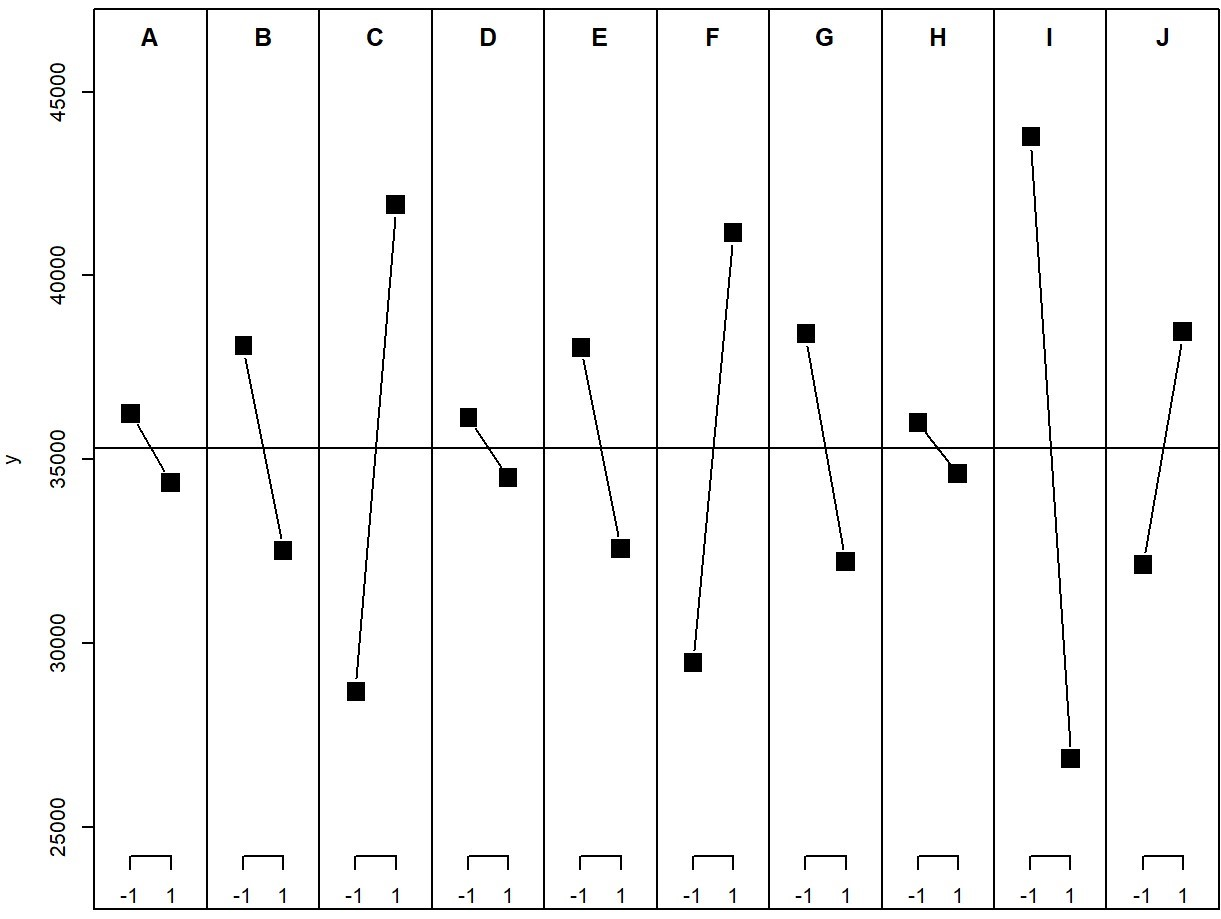
\includegraphics[scale = 0.6]{main}
\caption{Main Effects Plot}\label{fig:main}
\end{figure}

The factors that are most obviously different, visually speaking, are $C$, $F$, and $I$. Again, we need additional tests to solid the argument. In particular, both stepwise regression and backward selection procedures indicate that $C$, $F$, and $I$ are statistically significant in the ANOVA model containing all first-order terms. Implementation details are provided in Appendix \ref{app:step}. Moreover, we have the following ANOVA results for first-order terms in Table \ref{tab:anova1}, implemented in Appendix \ref{app:anova}. Note that the ANOVA \textit{p}-values for all factors are not significant at 5 percent significance level. On the other hand, the \textit{p}-values for factors $C$, $F$, and $I$ are close enough to 0.05, compared to the rest whose \textit{p}-values deviate heavily. Hence, we justify that factors $C$, $F$, and $I$ are active.

\begin{table}[h!]
\centering
\caption{Analysis of Variance for all First-Order Factors} 
\label{tab:anova1}
\resizebox{\textwidth}{!}{
\begin{tabular}{lccccc}
\toprule
\textbf{Source of Variation} & \textbf{Sum of Squares} & \textbf{Degrees of Freedom} & \textbf{Mean Square} & $\pmb{F_0}$ & \textbf{\textit{P}-Value} \\ 
\midrule
A & $\mathsf{14,135,880}$ & $\mathsf{1}$ & $\mathsf{14,135,880}$ & $\mathsf{0.074}$ & $\mathsf{0.797}$ \\
B & $\mathsf{124,527,952}$ & $\mathsf{1}$ & $\mathsf{124,527,952}$ & $\mathsf{0.648}$ & $\mathsf{0.457}$ \\
C & $\mathsf{700,758,290}$ & $\mathsf{1}$ & $\mathsf{700,758,290}$ & $\mathsf{3.646}$ & $\mathsf{0.114}$ \\
D & $\mathsf{10,598,320}$ & $\mathsf{1}$ & $\mathsf{10,598,320}$ & $\mathsf{0.055}$ & $\mathsf{0.837}$ \\
E & $\mathsf{120,120,664}$ & $\mathsf{1}$ & $\mathsf{120,120,664}$ & $\mathsf{0.625}$ & $\mathsf{0.465}$ \\
F & $\mathsf{546,886,110}$ & $\mathsf{1}$ & $\mathsf{546,886,110}$ & $\mathsf{2.846}$ & $\mathsf{0.152}$ \\
G & $\mathsf{153,852,120}$ & $\mathsf{1}$ & $\mathsf{153,852,120}$ & $\mathsf{0.801}$ & $\mathsf{0.412}$ \\
H & $\mathsf{7,813,926}$ & $\mathsf{1}$ & $\mathsf{7,813,926}$ & $\mathsf{0.041}$ & $\mathsf{0.848}$ \\
I & $\mathsf{1,143,446,322}$ & $\mathsf{1}$ & $\mathsf{1,143,446,322}$ & $\mathsf{5.950}$ & $\mathsf{0.059}$ \\
J & $\mathsf{160,067,701}$ & $\mathsf{1}$ & $\mathsf{160,067,701}$ & $\mathsf{0.833}$ & $\mathsf{0.403}$ \\
Error & $\mathsf{960,963,779}$ & $\mathsf{5}$ & $\mathsf{192,192,756}$ &  &  \\
Total & $\mathsf{3,943,171,064}$ & $\mathsf{15}$ &  &  &  \\
\bottomrule
\end{tabular}}
\end{table}

To conclude the preliminary examination, we have the following model specification in Table \ref{tab:spec} illustrating which variables should be included in or excluded from the analysis done previously.

\begin{table}[h!]
\centering
\caption{Model Specification} 
\label{tab:spec}
\begin{tabular}{lcccccccccc}
\toprule
\textbf{Variables} & $A$ & $B$ & $C$ & $D$ & $E$ & $F$ & $G$ & $H$ & $I$ & $J$ \\ 
\textbf{Model} & Out & Out & In & Out & Out & In & Out & Out & In & Out \\
\bottomrule
\end{tabular}
\end{table}

\subsection{General Analysis Procedure}
After determining the three active factors, we proceed to do a follow-up $2^3$ factorial experiment to investigate the interactions, as suggested in Section \ref{sec:general}. We first visually examine the interaction effects matrix for the three factors. The plots are shown in Figure \ref{fig:interaction}, implemented in Appendix \ref{app:plots}. The factor names are printed on the diagonal of the plot matrix. Note that the two lines for each plot (interaction) are unparallel. This may indicate a statistically insignificant conclusion for the interaction effects to be added to the model.

\begin{figure}[h!]
\centering
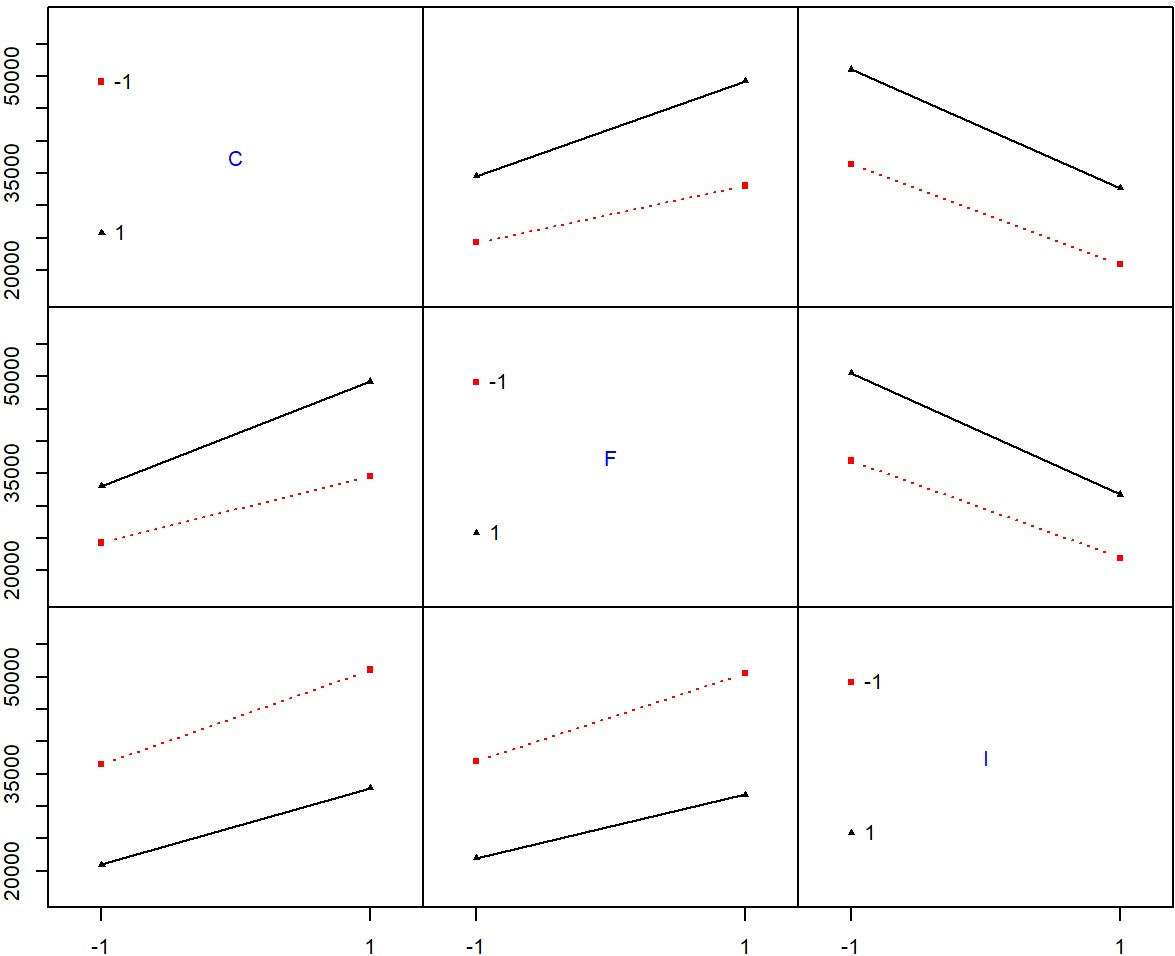
\includegraphics[scale = 0.6]{interaction}
\caption{Interaction Effects Matrix}\label{fig:interaction}
\end{figure}

To formally test the significance of the interaction terms, we build a three-factor ANOVA model for the three factors. The pooling of three-factor interaction is used here because we assume three-factor interactions are small concerning the main and two-factor interaction terms for unreplicated two-level studies. The complete ANOVA results with a decomposition of interaction sum of squares are shown in Table \ref{tab:anova2a} and \ref{tab:anova2b}. The implementation code is included in Appendix \ref{app:anova}. The \textit{p}-value of the interaction shows the insignificance to be added to the model. Hence, our final model contains the three first-order terms without interactions.

\begin{table}[h!]
\centering
\caption{Analysis of Variance for Significance of Regression and Interaction} 
\label{tab:anova2a}
\resizebox{\textwidth}{!}{
\begin{tabular}{lccccc}
\toprule
\textbf{Source of Variation} & \textbf{Sum of Squares} & \textbf{Degrees of Freedom} & \textbf{Mean Square} & $\pmb{F_0}$ & \textbf{\textit{P}-Value} \\ 
\midrule
Regression & $\mathsf{2,391,090,722}$ & $\mathsf{3}$ & $\mathsf{797,030,241}$ & $\mathsf{4.796}$ & $\mathsf{0.029}$ \\
Interaction & $\mathsf{56,438,583}$ & $\mathsf{3}$ & $\mathsf{18,812,861}$ & $\mathsf{0.113}$ & $\mathsf{0.950}$ \\
Error & $\mathsf{1,495,641,759}$ & $\mathsf{9}$ & $\mathsf{166,182,418}$ &  &  \\
Total & $\mathsf{3,943,171,064}$ & $\mathsf{15}$ &  &  &  \\
\bottomrule
\end{tabular}}

\caption{Decomposition of Interaction Sum of Squares} 
\label{tab:anova2b}
\begin{tabular}{lccccc}
\toprule
\textbf{Source of Variation} & \textbf{Sum of Squares} & \textbf{Degrees of Freedom} \\ 
\midrule
$C\times F$ & $\mathsf{34,488,777}$ & $\mathsf{1}$ \\
$C\times I$ & $\mathsf{7,813,926}$ & $\mathsf{1}$ \\
$F\times I$ & $\mathsf{14,135,880}$ & $\mathsf{1}$ \\
\bottomrule
\end{tabular}
\end{table}

The regression version of the three-factor ANOVA model can be stated as follows:
\begin{equation}\label{eq:model}
Y_i=\beta_{0}+\beta_{1}C_{i}+\beta_{2}F_{i}+\beta_{3}I_{i}+\epsilon_{i}.
\end{equation}
The implementation in Appendix \ref{app:anova} outputs the following regression equation:
\begin{equation}\label{eq:reg}
\hat{Y_i}=35309.318+6617.960\,C_{i}+5846.399\,F_{i}-8453.721\,I_{i}.
\end{equation}
The two widely used methods for assessing the overall adequacy of the model are multiple R-squared and adjusted R-squared. They are 0.6064 and 0.508, respectively. Tables \ref{tab:anova3a} and \ref{tab:anova3b} provide additional details on the significance of regression and its decomposition into sums of squares.

\begin{table}[h!]
\centering
\caption{Analysis of Variance for Significance of Regression} 
\label{tab:anova3a}
\resizebox{\textwidth}{!}{
\begin{tabular}{lccccc}
\toprule
\textbf{Source of Variation} & \textbf{Sum of Squares} & \textbf{Degrees of Freedom} & \textbf{Mean Square} & $\pmb{F_0}$ & \textbf{\textit{P}-Value} \\ 
\midrule
Regression & $\mathsf{2,391,090,722}$ & $\mathsf{3}$ & $\mathsf{797,030,241}$ & $\mathsf{6.162}$ & $\mathsf{0.00887}$ \\
Error & $\mathsf{1,552,080,342}$ & $\mathsf{12}$ & $\mathsf{129,340,028}$ &  &  \\
Total & $\mathsf{3,943,171,064}$ & $\mathsf{15}$ &  &  &  \\
\bottomrule
\end{tabular}}

\caption{Decomposition of Regression Sum of Squares} 
\label{tab:anova3b}
\begin{tabular}{lccccc}
\toprule
\textbf{Source of Variation} & \textbf{Sum of Squares} & \textbf{Degrees of Freedom} \\ 
\midrule
$C$ & $\mathsf{700,758,290}$ & $\mathsf{1}$ \\
$F$ & $\mathsf{546,886,110}$ & $\mathsf{1}$ \\
$I$ & $\mathsf{1,143,446,322}$ & $\mathsf{1}$ \\
\bottomrule
\end{tabular}
\end{table}

\subsection{ANOVA Diagnostics and Remedial Measures}
Model adequacy checking using the classical graphical methods enables researchers to decide if remedial measures are needed to improve the model effectiveness. Figure \ref{fig:residual} is the diagnostic residual versus fitted value plot. The diagnostic normal probability plot is provided in Figure \ref{fig:qq}. Appendix \ref{app:residual} shows the code to generate the plots.

\begin{figure}[h!]
\centering
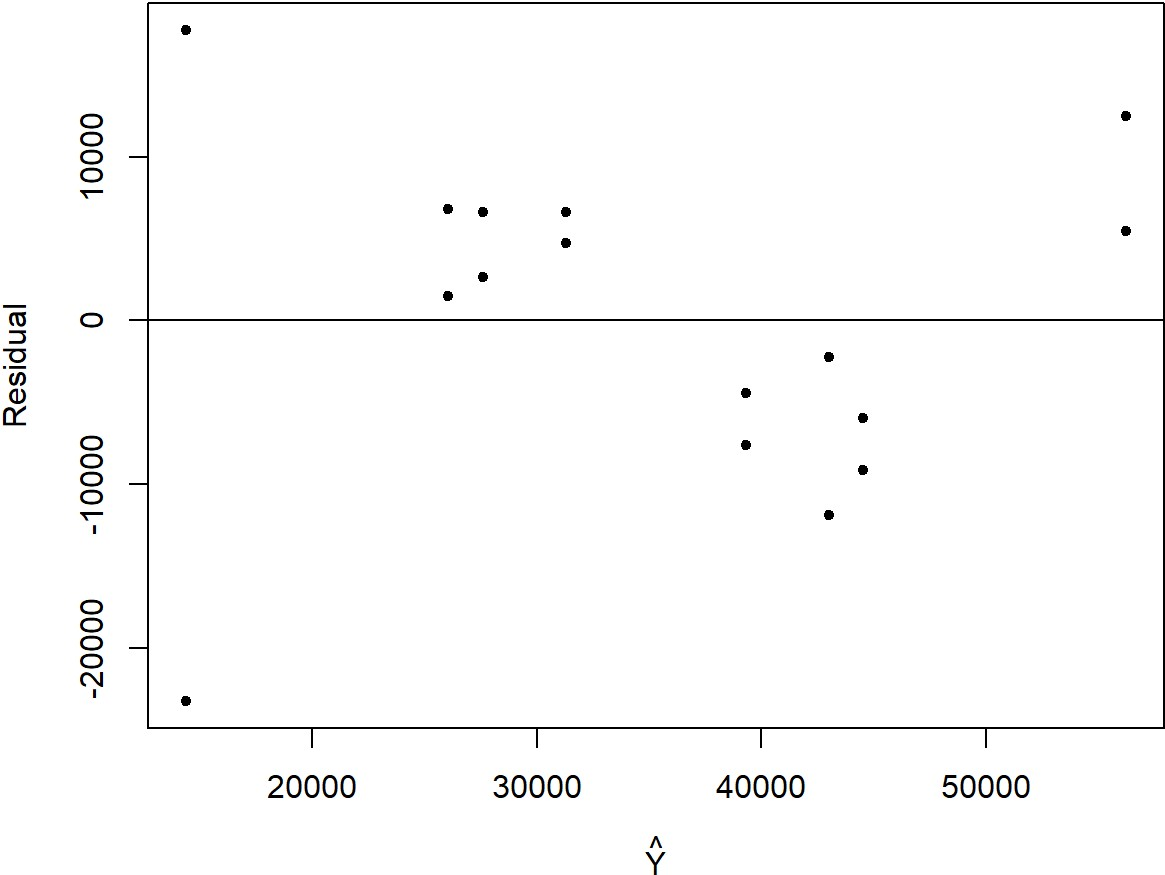
\includegraphics[scale = 0.6]{residual}
\caption{Residual against the Fitted Values}\label{fig:residual}
\end{figure}

\begin{figure}[h!]
\centering
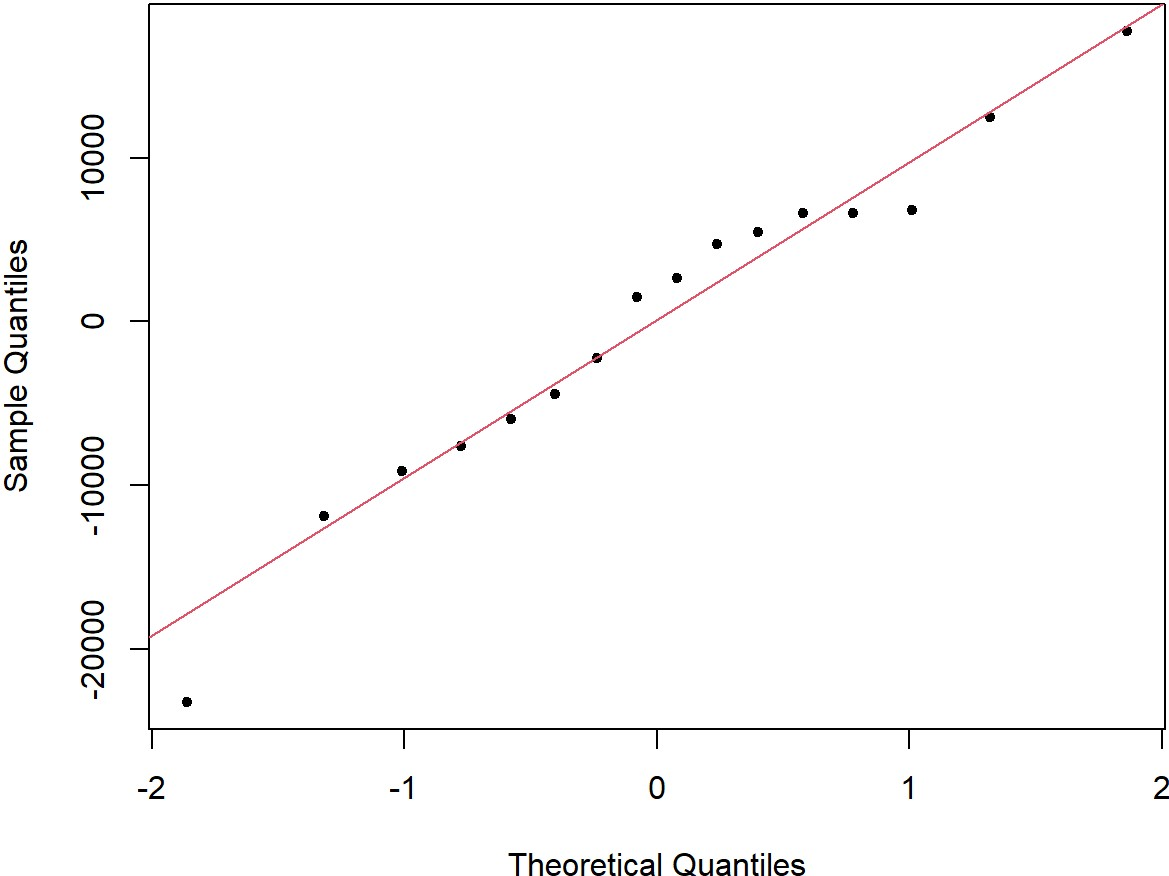
\includegraphics[scale = 0.6]{qq}
\caption{Normal Q-Q Plot}\label{fig:qq}
\end{figure}

As discussed previously in Section \ref{sec:diag}, we shall investigate every possible departure from the ANOVA model suggested by Kutner et al. \cite{bk:dae1} to finish ANOVA diagnostics.

\begin{description}
\item [Nonconstancy of Error Variance] \hfill \\ The residual plot against the fitted values in Figure \ref{fig:residual} shows no unusual pattern. Especially, since the sample size is comparatively small, it is normal that the residual scatters around zero for each factor level are slightly different. Thus, we claim the error variance is constant.

\item [Nonindependence of Error Terms] \hfill \\ Because randomization is enforced in the experiment, the assumption of error term independence is not violated. What is more, the nonindependence of error terms normally requires verification for experiments with time-related effects \cite{bk:dae1, bk:dae2}.

\item [Outliers] \hfill \\ Residual plots versus fitted values facilitate the detection of outliers. In particular, Figure \ref{fig:residual} reveals a structureless pattern. Moreover, due to the relatively small sample size for the resource constraints, a few observations that are seemingly different than other observations may be normal. Finally, Kutner et al. \cite{bk:dae1} recommend discarding possibly outlying observations only when the observations are identified as incorrectly measured or entered. In our case, we have no evidence to delete any values and thus, no remedial measures are needed to take place.

\item [Omission of Important Explanatory Variables] \hfill \\ This assumption automatically holds because of the background given in the current problem. If an investigation is required, residual analysis can also be applied to study if the model is adequate \cite{bk:dae1}. The residual plot shows no apparent assumption-deviation pattern.

\item [Nonnormality of Error Terms] \hfill \\ The normal Q-Q plot in Figure \ref{fig:qq} depicts a nicely straight line on the central values of the plot. Since the number of observations is relatively small, it is not unusual to have one or two extreme residuals deviating slightly from the straight line. Thus, we conclude the normality assumption is not violated.
\end{description}

\subsection{Statistical Inference}
Here, we present several important statistical inference results, as discussed in Section \ref{sec:si}. First, the \textit{p}-value for the test of regression, from Table \ref{tab:anova3a}, is 0.00887. This implies that we reject the null hypothesis that none of the regressors contribute significantly to the model at 5 percent level of significance. Furthermore, recall the point estimates for regression coefficients in Equation \ref{eq:reg} are $\hat{\beta_0}=35309.318$, $\hat{\beta_1}=6617.960$, $\hat{\beta_2}=5846.399$ and $\hat{\beta_3}=-8453.721$, respectively. We obtain the following 95 percent confidence intervals for $\beta_j$s:
\begin{align*}
29114.53 \leq & \beta_0 \leq 41504.11 \\
423.173 \leq & \beta_1 \leq 12812.75 \\
-348.388 \leq & \beta_2 \leq 12041.19 \\
-14648.51 \leq & \beta_3 \leq -2258.93
\end{align*}
 
We can predict the mean of the response by the settings of the control variables. For example, suppose we are interested in the response for $C=1$, $F=-1$, and $I=1$. We have $\hat{Y_h}=27627.158$. The 95 percent prediction interval for $Y_{h\text{(new)}}$: $-76.774 \leq Y_{h\text{(new)}} \leq 55331.09$. The 95 percent confidence interval for $\mu_{Y}$: $15237.58 \leq \mu_{Y} \leq 40016.73$. The calculation implementation is shown in Section \ref{app:si}.

\section{Discussion}\label{sec:discussion}
The main advantage of applied statistical methods is to increase objectivity in a variety of decision-making scenarios \cite{bk:dae2}. In this paper, we have been improving our confidence in designing an experiment and modeling the given data. However, the conclusions do not prove factors $C$, $F$, and $I$ have particular effects. They only serve as guidelines to increase the reliability and validity of results. The following subsections provide additional insights into different perspectives of our research.

\subsection{Unreplicated Two-Level Studies}\label{sec:rep}
Montgomery \cite{bk:dae2} proposes risk of conducting an unreplicated experiment is that the fitting model may be pure noise. That is, the estimated factor effects may be close to zero. Therefore, the experimenter may falsely conclude the insignificance of the factors. If the variability of the response is smaller, the probability of an erroneous conclusion will be smaller \cite{bk:dae2}.

\subsection{Advantages of Orthogonal Coding}\label{sec:oe}
Recall that $\pmb{X}$ is the regressor matrix, also called the design matrix, storing all factor values. When a balanced factorial experiment is carried out at two levels for each factor and a $\pm 1$ orthogonal coding is employed, the $\pmb{X}^{T}\pmb{X}$ matrix is greatly simplified. Consider the $2^{k}$ factorial design we have discussed with one replication in Section \ref{sec:dsg}. The $\pmb{X}^{T}\pmb{X}$ matrix is simplified because:

\begin{itemize}
\item Any two columns of the $\pmb{X}$ matrix are orthogonal; that is, $\pmb{X}^{T}_{q}\pmb{X}_{q'}=0$. 

\item The sum of squares of the elements in each column, $\pmb{X}^{T}_{q}\pmb{X}_{q}$, is always $2^{k}$. It leads for balanced two-level factorial designs to a diagonal $\pmb{X}^{T}\pmb{X}$ matrix. 
\end{itemize}

Thus, the least squares and maximum likelihood estimators of $\pmb{\hat{\beta}}=(\pmb{X}^{T}\pmb{X})^{-1}\pmb{X}^{T}\pmb{Y}$ can be written in a simple form of $\frac{1}{2^{k}}\pmb{X}^{T}\pmb{Y}$ \cite{bk:dae1}. Furthermore, if we write the regression model as $\pmb{Y}=\pmb{X}\pmb{\beta}+\pmb{\epsilon}=\pmb{X}_{1}\pmb{\beta}_{1}+\pmb{X}_{2}\pmb{\beta}_{2}+\pmb{\epsilon}$, the sum of squares of $\pmb{\beta}_{1}$ and the sum of squares of $\pmb{\beta}_{2}$ measure the contribution of the regressors in $\pmb{X}_1$ and $\pmb{X}_2$, respectively, to the model unconditionally. In other words, if the independent variables are orthogonal, we can uniquely determine each variable's effects on the model. Because of this, researchers are often willing to have orthogonal coding regressors in their data collection experiments \cite{bk:ilra}.

\subsection{Resolution}\label{sec:resolution}
There is a trade-off between the resolution level and the number of observations in a study. For higher resolutions, the assumptions of including unimportant interactions in the model become less restrictive \cite{bk:dae2}. In this paper, we used the one-sixty-fourth fraction of the $2^{10}$ factorial design with resolution \MakeUppercase{\romannumeral 3} in 16 runs. It is of interest for experimenters to choose the highest possible resolution of design \cite{bk:dae1, bk:dae2}. Recall the possible alternatives we have are $2^{10-3}_{\text{\MakeUppercase{\romannumeral 5}}}$, $2^{10-4}_{\text{\MakeUppercase{\romannumeral 4}}}$ and $2^{10-5}_{\text{\MakeUppercase{\romannumeral 4}}}$ with 128, 64 and 32 runs, respectively. Therefore, for future research, we can choose a $2^{10-3}_{\text{\MakeUppercase{\romannumeral 5}}}$ design if we believe the loss of sacrificing higher-order interactions information outweighs the cost of runs, given sufficient resources.

\subsection{Plots of Estimated Factor Level Means}\label{sec:plots}
Kutner et al. \cite{bk:dae1} suggest the following four types of plots to informally inspect the factor level effects: a line plot, a bar graph, a main effects plot, and a normal probability plot. We use the main effects plot to visualize. Remark that the four plots themselves do not provide any information on the standard errors. Thus, we cannot make a solid conclusion that the differences are statistically significant between the factor level means. Bar-interval graph and interval plot are enhanced bar graph and main effects plot, respectively, such that the confidence limits for each factor level mean are included \cite{bk:dae1}. Also, note that a normal probability plot is a suitable informal examination when the sample sizes are equal and the number of factors is sufficiently large, such as greater than or equal to 10 \cite{bk:dae1}. Therefore, we can also adopt the normal probability plot in this paper to visualize the factor level means.

\appendix
\section{Technical Implementation in \texttt{R}}\label{sec:app}

\subsection{Factorial Design Generation}\label{app:fdg}
Computer statistical software is broadly used to assist experimenters in choosing and building experimental designs \cite{bk:dae2}. The following code builds a $2^{10-6}_{\text{\MakeUppercase{\romannumeral 3}}}$ statistical design in random order to follow the randomization principle discussed in Section \ref{sec:dsg}. The complete alias relationship for the design used in this paper is included in Table \ref{tab:alias}.
\begin{file}[dae.r]
\begin{lstlisting}[language = R]
library(FrF2)
dsg <- 
   FrF2(nruns = 16, nfactors = 10, factor.names = LETTERS[1:10],
        generators = c("ABC", "BCD", "ACD", "ABD", "ABCD", "AB"), 
        seed = 123)
summary(dsg)
\end{lstlisting}
\end{file}

\begin{table}[h!]
\caption{Alias Relationship for $2^{10-6}$ Fractional Factorial Design}\label{tab:alias}
\vspace{-1.8ex}
\noindent\rule{\textwidth}{0.08em}
$2^{10-6}$; 1/64 fraction of 10 factors in 16 runs\hfill \textbf{Resolution \MakeUppercase{\romannumeral 3}}\\
\centerline{\underline{Design Generators}}
\[
E = ABC\quad F = BCD\quad G = ACD\quad H = ABD\quad I = ABCD\quad J = AB
\]
\centerline{\underline{Defining relation}}
\begin{align*}
0 &= ABCE = BCDF = ADEF = ACDG = BDEG = ABFG = CEFG = ABDH \\
  &= CDEH = ACFH = BEFH = BCGH = AEGH = DFGH = ABCDEFGH = ABCDI \\
  &= DEI = AFI = BCEFI = BGI = ACEGI = CDFGI = ABDEFGI = CHI \\
  &= ABEHI = BDFHI = ACDEFHI = ADGHI = BCDEGHI = ABCFGHI \\
  &= EFGHI = ABJ = CEJ = ACDFJ = BDEFJ = BCDGJ = ADEGJ = FGJ \\
  &= ABCEFGJ = DHJ = ABCDEHJ = BCFHJ = AEFHJ = ACGHJ = BEGHJ \\
  &= ABDFGHJ = CDEFGHJ = CDIJ = ABDEIJ = BFIJ = ACEFIJ = AGIJ \\
  &= BCEGIJ = ABCDFGIJ = DEFGIJ = ABCHIJ = EHIJ = ADFHIJ \\
  &= BCDEFHIJ = BDGHIJ = ACDEGHIJ = CFGHIJ = ABEFGHIJ    
\end{align*}
\centerline{\underline{Aliases}}
\begin{align*}
A &= FI = BJ\qquad I = DE = AF = BG = CH \\
B &= GI = AJ\qquad J = AB = CE = FG = DH \\
C &= HI = EJ\qquad AC = BE = DG = FH \\
D &= EI = HJ\qquad AD = EF = CG = BH \\
E &= DI = CJ\qquad AE = BC = DF = GH \\
F &= AI = GJ\qquad AG = CD = BF = EH = IJ \\
G &= BI = FJ\qquad AH = BD = CF = EG \\
H &= CI = DJ
\end{align*}\vspace{-1.8ex}
\centerline{2 blocks of 8:\,$AG = CD = BF = EH = IJ$}
\noindent\rule{\textwidth}{0.08em}
\end{table}

\subsection{Analysis of Variance and Linear Model}\label{app:anova}
Suppose we have input the dataset in Table \ref{tab:dsg} named \texttt{data} in the code. We can obtain ANOVA and linear model results using functions \texttt{aov()} and \texttt{lm()}, respectively. Table \ref{tab:anova1} is the ANOVA output from \texttt{anova(aov1)}; Tables \ref{tab:anova2a} and \ref{tab:anova2b} are from \texttt{anova(aov2)}; Tables \ref{tab:anova3a} and \ref{tab:anova3b} are from \texttt{anova(aov3)}. \texttt{summary()} provides summaries of model fitting functions such as model function coefficients, \textit{F}-statistic and its \textit{p}-value. Equation \ref{eq:reg} can be obtained from the summary of \texttt{lm3}.
\begin{file}[dae.r]
\begin{lstlisting}[language = R]
aov1 = aov(y ~ ., data = data)
anova(aov1)

aov2 = aov(y ~ C*F*I, data = data)
anova(aov2)

aov3 = aov(y ~ C + F + I, data = data)
anova(aov3)

lm3 = lm(y ~ C + F + I, data = data)
summary(lm3)
\end{lstlisting}
\end{file}

\subsection{Stepwise Regression}\label{app:step}
Stepwise selection and backward elimination can be done by the function \texttt{step()}. Note that, by default, \texttt{R} uses the Akaike information criterion (AIC). That is, \texttt{k = 2} is used by default in the following code, where \texttt{k} is the multiple of the number of degrees of freedom used for the penalty. To use the BIC, we simply have \texttt{k = log(nrow(data))} instead.
\begin{file}[dae.r]
\begin{lstlisting}[language = R]
step(aov1, k = log(nrow(data)))

step(aov1, direction = "backward", k = log(nrow(data)))
\end{lstlisting}
\end{file}

\subsection{Main Effects Plot and Interaction Effects Matrix}\label{app:plots}
\texttt{FrF2} package has two useful functions, \texttt{MEPlot()} and \texttt{IAPlot()}, to graphically display the main effects plot and the interaction plots, shown in Figure \ref{fig:main} and Figure \ref{fig:interaction}, respectively.
\begin{file}[dae.r]
\begin{lstlisting}[language = R]
MEPlot(aov1, main = NULL)

IAPlot(aov2, main = NULL)
\end{lstlisting}
\end{file}

\subsection{Residual Analysis}\label{app:residual}
Residual analysis, discussed in Section \ref{sec:diag}, is one the most important procedure to evaluate model adequacy in applied statistics. We present a residual plot versus the fitted values shown in Figure \ref{fig:residual} and a normal probability plot of the residuals in Figure \ref{fig:qq}. \texttt{resid()} calculates the residuals for all observations from the linear model. The \texttt{plot()} and \texttt{abline()} functions plot the fitted values of the linear model with the residuals to visualize the random pattern. The normal Q-Q plot is created using the traditional commands \texttt{qqnorm()} and \texttt{qqline()}.
\begin{file}[dae.r]
\begin{lstlisting}[language = R]
res = resid(lm3)

plot(fitted(lm3), res, xlab = expression(hat(Y)), 
     ylab = "Residual", pch = 20)
abline(0, 0)

qqnorm(res, main = NULL, pch = 20)
qqline(res, col = 2)
\end{lstlisting}
\end{file}

\subsection{Confidence and Prediction Intervals}\label{app:si}
Statistical inference results can be obtained in \texttt{R}. For confidence intervals of regression coefficients, \texttt{confint()} directly provides the $(1-\alpha)\%$ confidence intervals for all coefficients (95 percent confidence interval by default). To obtain confidence and prediction intervals of the mean of a new response, we first predict the response given the factor values. Then the interval estimations are given using \texttt{predict()} with the type of interval estimation specified. The following code retrieves the predictions of all possible combinations of the factor values with interval estimations returned. 
\begin{file}[dae.r]
\begin{lstlisting}[language = R]
confint(lm3)

pred_data <- expand.grid(C = c(-1, 1), F = c(-1, 1), I = c(-1, 1))
predict(lm3, newdata = pred_data, interval = "confidence")
predict(lm3, newdata = pred_data, interval = "prediction")
\end{lstlisting}
\end{file}

\bibliographystyle{abbrv}
\bibliography{refs}

\end{document}
